
\begin{frame}{Proof Sketch}

The actual proof is between $E^n$ and $E^{n-1}$, which gives inductively
that a function in $E^n$ can be represented with functions in $E$.

To allow for nice figures, we will show that for any $f:E^2\rightarrow\mathcal{R}$
there are $\phi_{0..4}:\mathcal{R}\rightarrow\mathcal{R}$
and $\psi_{0..4,1..2}:E\rightarrow\mathcal{R}$ such that:
$$
f(x_1,x_2)=\sum_{q=0}^4\phi_q\left(\psi_{q,1}\left(x_1\right)+\psi_{q,2}\left(x_2\right)\right)
$$

The proof proceeds in three steps:
%
\begin{itemize}
\item Cover the unit square
\item Construct the inner functions $\psi$
\item Construct the outer functions $\phi$
\end{itemize}
\end{frame}



\begin{frame}{Proof Sketch Step 1: Cover the unit square}

For any integer $k>0$, we can construct $k$ non-overlapping intervals
in $E$ with length less than $1/k$
As $k>0$ gets larger, the length of each interval gets smaller; at the
limit the length of each interval will approach zero.

\vskip 1em

Fix a value for $k$.

\vskip 1em

Let $A_{k,1}$ be the union of such intervals for $p=1$ (i.e., for the
first input of $f$).

\vskip 1em

We repeat the process to make one such union $A_{k,1}^q$ for each
value of $q = 0..2n$. All $A_{k,1}^q$ are one
\emph{family} and all $A_{k,2}^q$ are another family. There are
$n=2$ families.

\end{frame}



\begin{frame}{Proof Sketch Step 1: Cover the unit square}

\textcolor{blue!50!black}{Every $x\in E$ is contained in no less than $2n$ (here, 4) members of the family}

\vskip 1 em

The families can always be constructed so that the gaps of their
members do not intersect:

\vskip 1 em

\begin{tabular}{lccccccccccccccc}
\hline
$A_{k,1}^0$ & x & x & x & x & x & x &   & x & x & x & x & x & x &   & x \\ 
\hline
$A_{k,1}^1$ &   & x & x & x & x & x & x &   & x & x & x & x & x & x &   \\
\hline
$A_{k,1}^2$ & x &   & x & x & x & x & x & x &   & x & x & x & x & x & x \\
\hline
$A_{k,1}^3$ & x & x &   & x & x & x & x & x & x &   & x & x & x & x & x \\
\hline
$A_{k,1}^4$ & x & x & x &   & x & x & x & x & x & x &   & x & x & x & x \\
\hline
\end{tabular}  
\vskip 1 em

so that any point in $E$ will be contained in at most one gap.

\end{frame}



\begin{frame}{Proof Sketch Step 1: Cover the unit square}

\begin{itemize}

\item Replicate the family $A_{k,1}^q$ into $A_{k,2}^q$ \vspace{0.5em}

\item For each $q$, constuct $S_k^q$, the union of the non-overlapping
  squares $A_{k,1}^q \times A_{k,2}^q$ \vspace{0.5em}

\item Any point in $E^2$ will be contained in at most one gap in each
  dimention, so will be contained in at least $2n+1-n = n+1$
  intervals \vspace{0.5em}

\end{itemize}
\vskip 1em

\textcolor{blue!50!black}{%
  The system of all rectangles $S_k^q, q=0..2n$ covers the unit square
  $E^2$ so that every point in $E^2$ is covered at least $n+1$ times.
}

\end{frame}



\begin{frame}{Proof Sketch Step 2: Construct the inner functions}

\begin{columns}

  \begin{column}{7cm}

  For given $k,q$, it is always possible to construct a series of
  constants $\lambda_i$ such that:

  $$
  \lambda_i < \lambda_{i+1} \leq \lambda_i + \frac{1}{2^k}
  $$

  and a function $\psi_1$ mapping inputs from the
  $A_{k,1}^q$ intervals to the corresponding $\lambda$ intervals.

  \vskip 1em

  Any continuous function will do, but let's say its a step function
  with linear connections across gaps, so that it's continuous and
  monotonic increasing.

  \end{column}

  \begin{column}{6.5cm}
  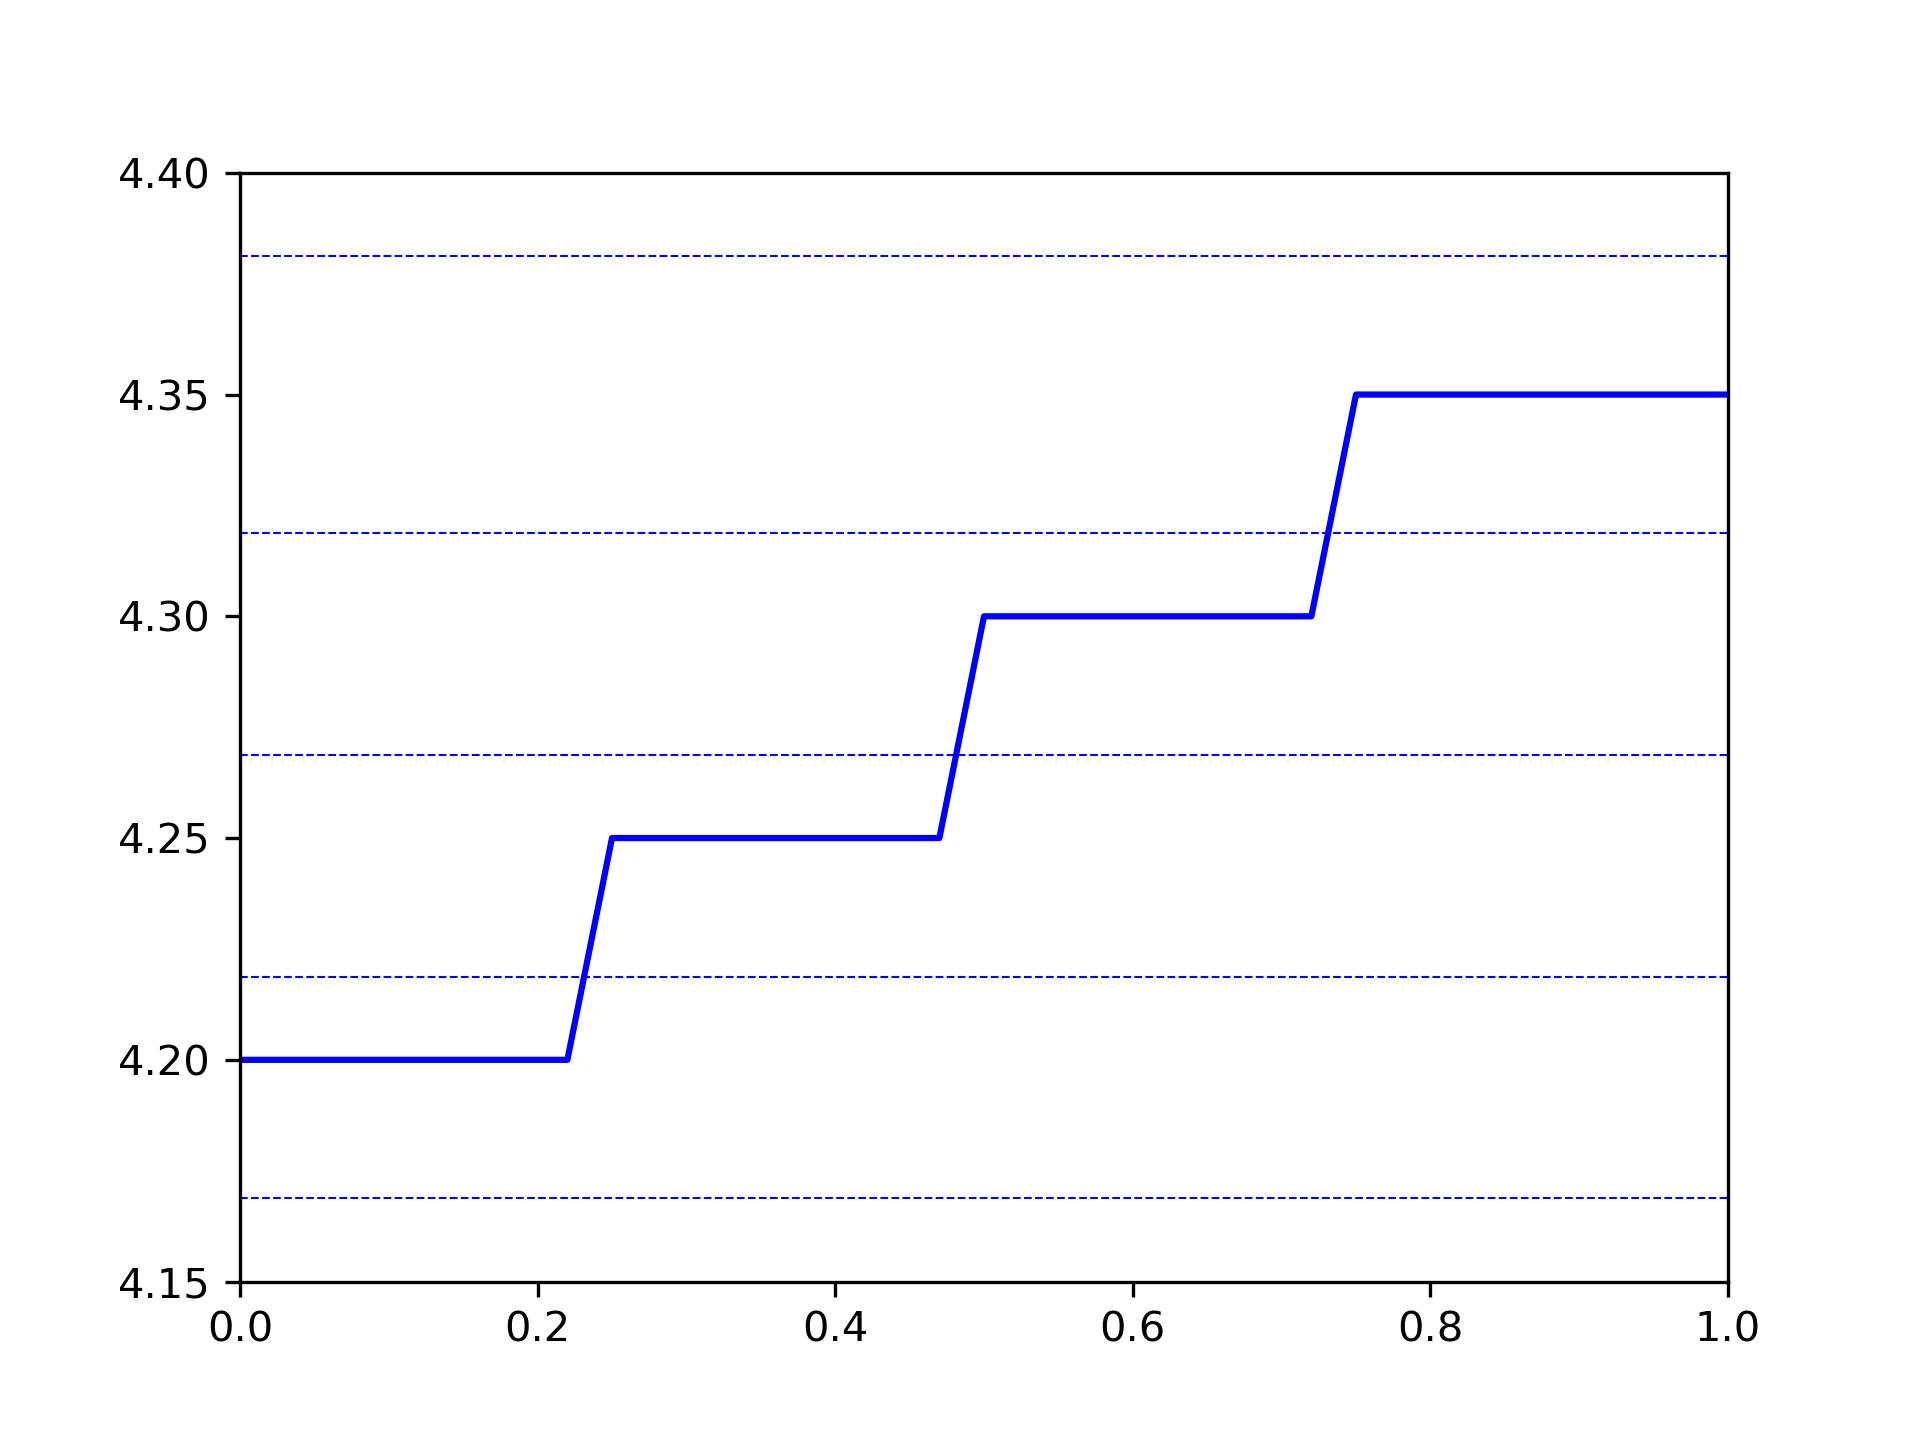
\includegraphics[width=6cm]{contents/images/kat_psi1}

  For $k=4$, four non-overlapping intervals and
  the corresponding `lanes' defined by the $\lambda$ series.
  \end{column}

\end{columns}

\end{frame}



\begin{frame}{Proof Sketch Step 2: Construct the inner functions}

Construct a similar series $\mu_i$ for the second dimension.
Then:
$$
\lambda_i+\mu_i < \lambda_{i+1}+\mu_{i+1} \leq \lambda_i + \mu_i + 2\frac{1}{2^k}
$$
so an $\epsilon_k < 2^{-k}$ can be found such that the closed intervals
$\left[ \lambda_i+\mu_i , \lambda_i+\mu_i+2\epsilon_k \right]$
do not intersect.

\vskip 1em

Since they do not intersect, we can apply the same logic as before to
construct two functions $\psi_1,\psi_2$
such that their addition maps elements from the $S_k$ squares
we constructed before, to values within these intervals:

$$
\mbox{For each } x_1,x_2\in S_k^q,
\psi_1(x_1)+\psi_2(x_2) \in \left[ \lambda_i+\mu_i , \lambda_i+\mu_i+2\epsilon_k\right]
$$

\end{frame}



\begin{frame}{Proof Sketch Step 2: Construct the inner functions}

\begin{columns}

  \begin{column}{7cm}
  There are many solutions, but Sprecher's (1972) formulation gives us
  something we can visualize:
  \vskip 1em
  A grid of non-overlapping \quotes{platforms}, linearly connected at the
  gaps, all having different $z$, so that each $z$ maps to exactly
  one $S_k$ or to a gap.
  \end{column}

  \begin{column}{6.5cm}
  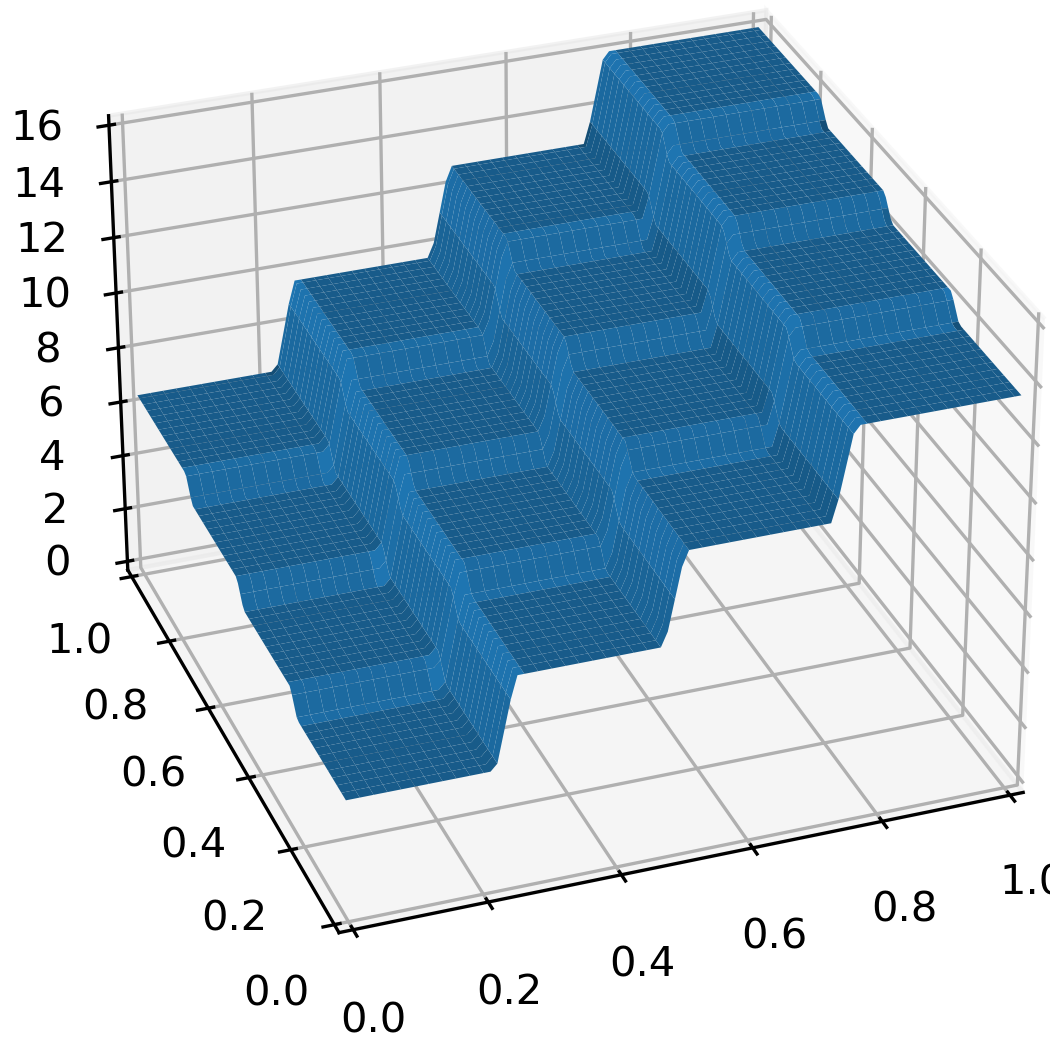
\includegraphics[width=6cm]{contents/images/kat_psi3}
  \end{column}

\end{columns}

\end{frame}



\begin{frame}{Proof Sketch Step 2: Construct the inner functions}

Reminder from Step 1:
\vspace{0.5em}
\begin{itemize}
\item For each $q=0..2n$, we constucted a family of non-overlapping
  squares $S_k^q$
\item Every point in $E^2$ is covered by at least $n+1$ squares
\end{itemize}

\vskip 1em

So we repeat all the above for all $q$ to create $2n+1$ different
$n$-tuples of $\psi$ functions.

\vskip 1em

\begin{itemize}
\item For each $q$, we have created a mapping from some values of
  $\psi_1(x_1)+\psi_2(x_2)$ to a $S_k^q$. The rest of the possible values
  of $\psi_1(x_1)+\psi_2(x_2)$ might be over a gap, but:
\item For each $x_1,x_2\in E^2$, at least $n+1$ of the $q$ families are not
  gaps
\end{itemize}

\end{frame}



\begin{frame}{Proof Sketch Step 3: Construct the outer functions}

All the pieces are now in place:
\vspace{0.5em}
\begin{itemize}
\item We have an `index' from $\psi_1(x_1)+\psi_2(x_2)$ to squares
  restricting the possible values of $x_1,x_2$. The size of the
  squares gets smaller as $k$ gets larger. \vspace{0.4em}
\item We can construct a function $f_k$ that simply `memorizes' how to
  approximate the value of the original $f$ from the sum of $\phi_p$ \vspace{0.3em}
  \begin{itemize}
  \item all pairs in the unit square are covered
  \item $f_k$ knows the neighbourhood of the $x_1,x_2$ values despite the fact
    that only sees sums
  \item $f_k$ can estimate $f$ with some error bounded by an
    expression denominated by $k$
  \end{itemize} \vspace{0.4em}
\item At the limit, there is no error
\end{itemize}

\vskip 0.8em

\textcolor{blue!50!black}{%
  Unlike the $\psi$ functions, we have no intuitions whatsoever
  about what the $\phi$ functions look like or how to construct them.
}

\end{frame}



\begin{frame}{Some More Thoughts}

There are many ways to pack two real numbers into one and then define
the function that unpacks the original numbers and applies $f$.
Here is one packing schema:

\vskip 1em

\begin{center}

  \begin{tabular}{l}
    0.42 \\
    0.31415926$\dots$ \\
    \hline
    0.4321040105090206$\dots$ \\
  \end{tabular}
  \end{center}

\vskip 0.5em

The Kolmogorov-Arnold therom tells us that it is possible to find a
\textbf{continuous} function that does the same
\vspace{0.5em}
\begin{itemize}
\item 'Continuous' sounds like a positive quality, but many
  `pathological' functions are nominally continuous
\item Under this light, we consider the claim that addition is the
  only multi-variate function strictly speaking valid, but over-hyped
\end{itemize}

\end{frame}



\begin{frame}{Some More Thoughts}

Kudos to Kolmogorov and Arnold for:
\vspace{0.5em}
\begin{itemize}
\item Anticipating modern ML: As long as it fits the data, it doesn't
  matter if the model captures the actual structures that generate the data \vspace{0.5em}
\item Anticipating modern ML II: In the executive summary, over-hype
  the significance of the result \vspace{0.5em}
\item Anticipating that multiple arguments can be passed as one complex
  \strong{record} a couple of years before COBOL \vspace{0.5em}
\item Making people reconsider the definition of \strong{function complexity}
\end{itemize}

\end{frame}



\begin{frame}{Post-KART}

\begin{itemize}
\item Hilbert's intuition about not being able to represent more
  complex functions by algebraically combining simpler functions remains valid:
  \begin{itemize}
  \item It obviously remains open for algebraic functions
  \item Its essense holds for any function, except that the K-A
    Representation Theorem proves that using the number of arguments
    to define complexity is wrong
  \item Vitushkin~(2004) gives a compelling argument
  \end{itemize}
\vspace{0.5em}
\item Hecht-Nielsen (1987) notes the similarity between Sprecher's
  formulation and NNs and speculates that NN training can be used to
  construct $\phi$, but Girosi \& Poggio (1989) point out that we know
  $\phi$ are not smooth (Vitushkin \& Henkin, 1967) and cannot be
  learnt.
\vspace{0.5em}
\item Schmidt-Hieber (2021) gives a good overview of the ways the KART
  has interacted with the ML community.
  
\end{itemize}

\end{frame}
